\chapter{Introduction}
\graphicspath{{foto/Chap1/}}
\section{Introduction to the laboratory experience}
This project aims to estimate the characteristics of a Register File based on Traditional Planar Transistors through a MATLAB script.

The outputs of the model are:
\begin{itemize}
\item Delay during read and write operations
\item Power consumption of a read operation
\item Power consumption of a write operation
\item Area and Volume
\end{itemize}

\section{Structure explanation}
It has been chosen to analyze a structure consisting of two read ports and a write port. A typical SRAM cell is made up of six MOSFETs, two of which are pass transistors, connecting the cell to the two complementary bit lines and to the word line that activates it. Since we need to design a three port register file, we add four more pass transistor, two for each word line. Each bit in a SRAM is stored on four transistors (P1, P2, N1, N2) that form two cross-coupled inverters. This storage cell has two stable states which are used to denote 0 and 1. Each couple of pass transistor is controlled by its own word line to allow parallel reading and writing operation; we assume, however, that only one operation at a time can be performed on a single memory cell. The structure analysed includes also some \textit{Decoders} and \textit{Pass transistors} used to select the correct word in the correct memory block, and some \textit{Sense Amplifier} used to recognize the value of the memory cells in a faster way. A more complete explanation is given in the Chapter 2; in fig. \ref{fig:reg_file} is shown a block structure of this Register File, while in fig. \ref{fig:cell_structure} is shown the structure of the memory cell adapted to support two read ports and one write port. 

	\begin{figure}[H] 
		\begin{center}
			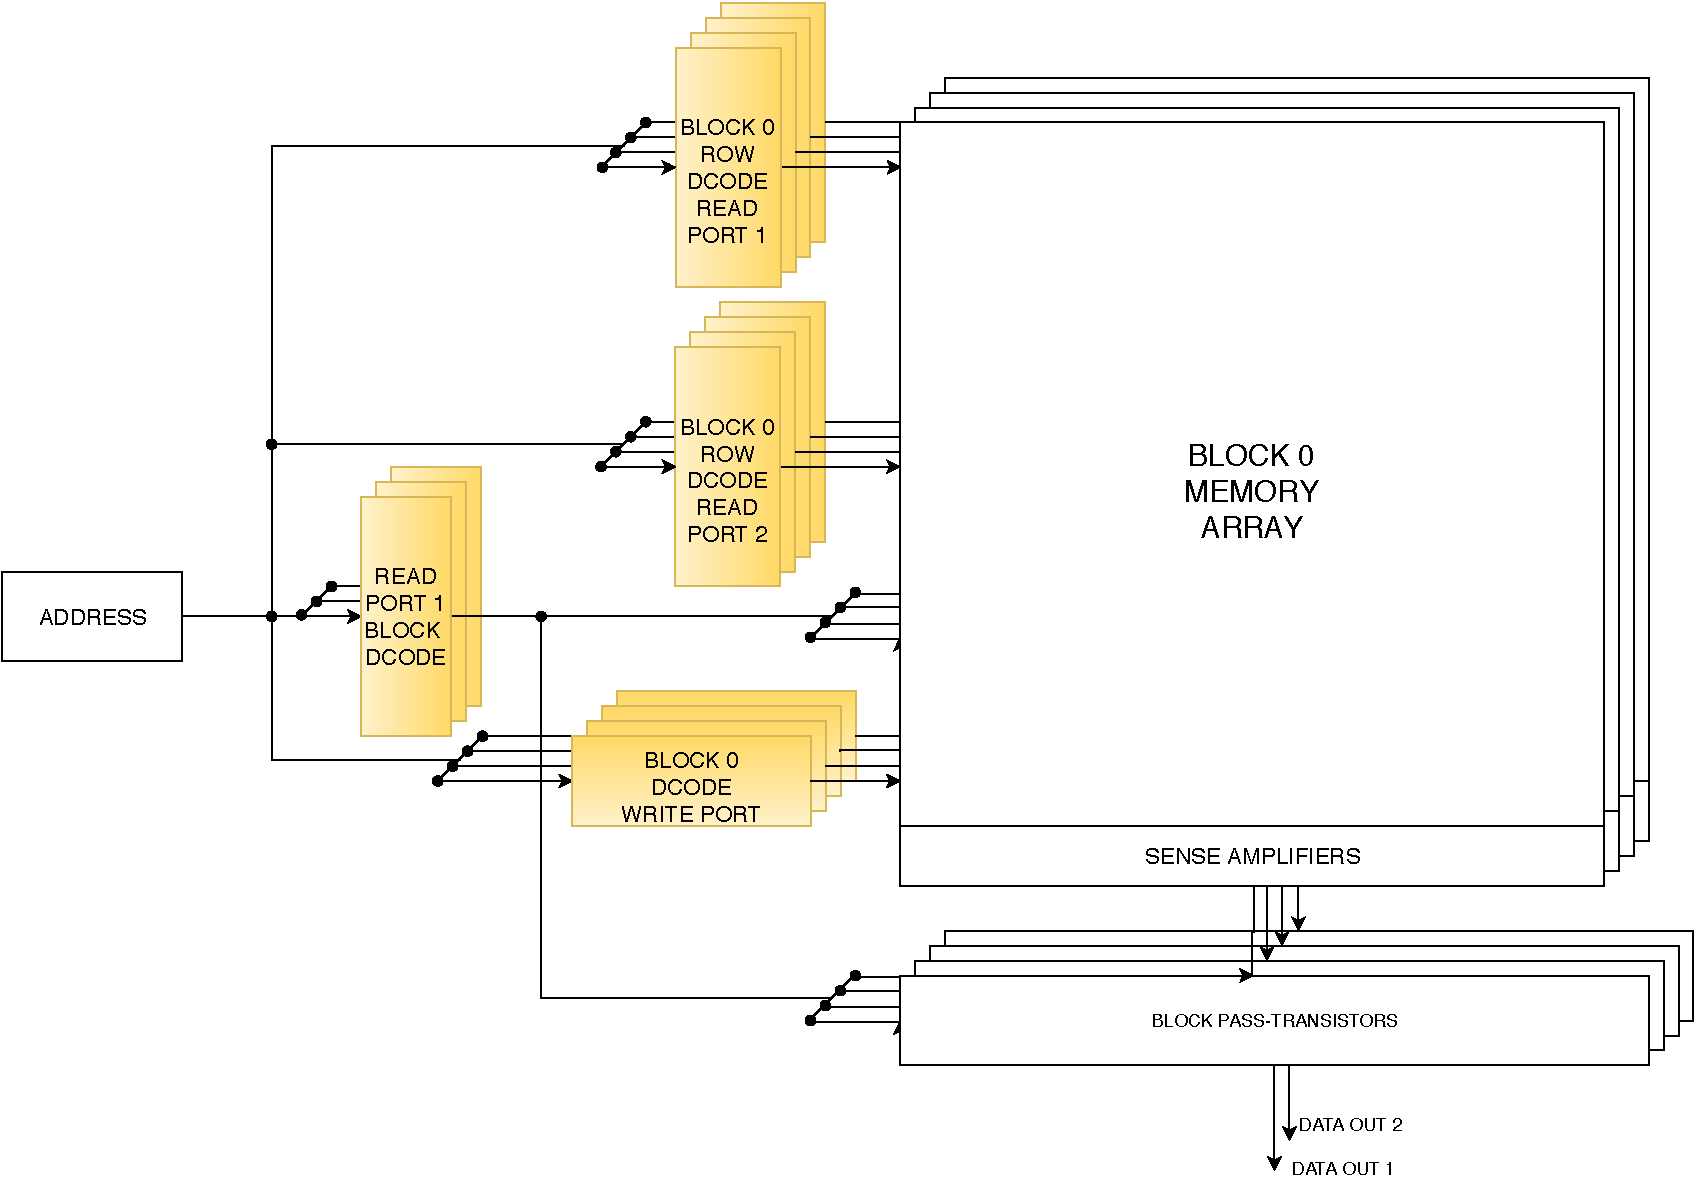
\includegraphics[scale=0.4]{REG_FILE-GENERAL_SCHEME}
		\end{center}
		\caption{Block structure of the register file} 
		\label{fig:reg_file}
	\end{figure}
	
	\begin{figure}[H] 
		\begin{center}
			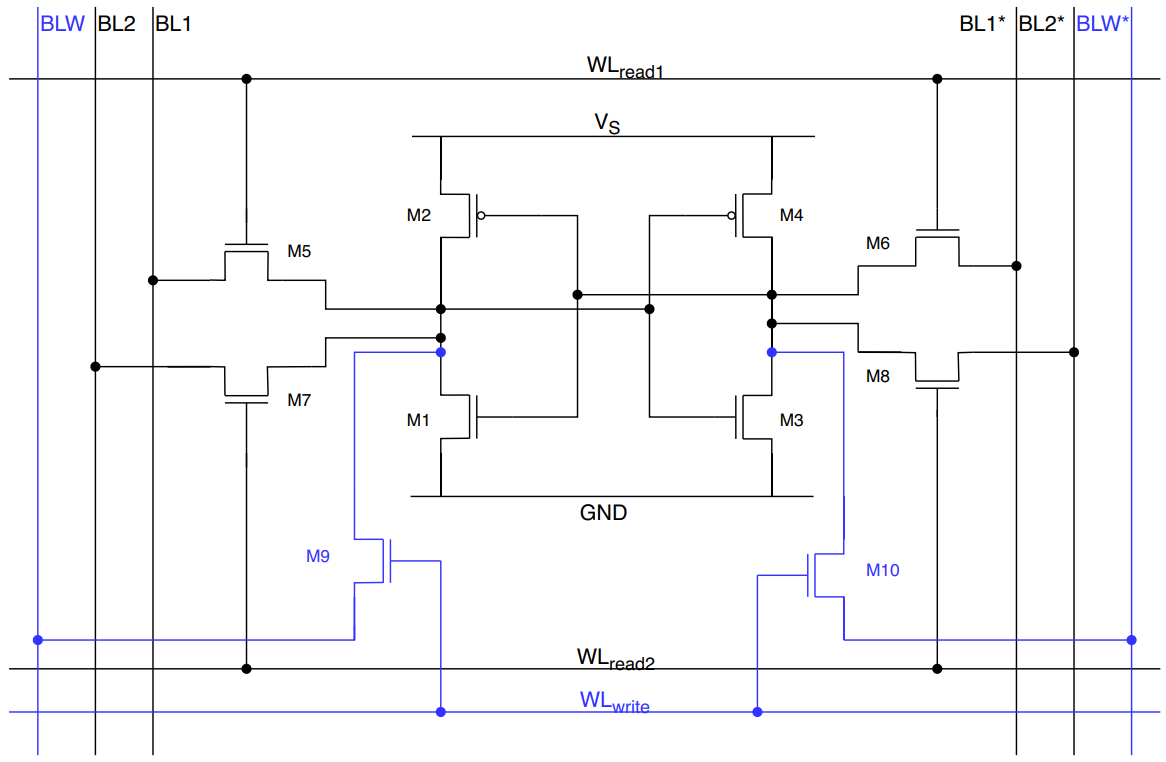
\includegraphics[scale=0.3]{sramcell.png}
		\end{center}
		\caption{Structure of a single SRAM cell} 
		\label{fig:cell_structure}
	\end{figure}	

\section{Behaviour of the memory}
The behaviour of the memory can be described in three operation.

\textbf{Precharge} is the initial state to perform a read or write operation. Actually the precharged bitlines are needed only during a read operation, but the precharge operation is done at the end of each read/write cycle to simplify the control of the memory. During the precharge state, bitlines are biased at a certain voltage to speed up subsequent operations.

\textbf{Read} operation. During this operation, unselected blocks are electrically disconnected by the block decoder. The address of the word to be read is divided into two fields: block address and row address. In general also a column address should be needed, but since we decided to realize memory arrays with parallelism equal to the width of a single word, a column decoder is not needed. According to the active read port $i$ (here $i$ goes from 1 to 2, since the third and last port is a write port), the corresponding block decoder $i$ selects the block, while all the row decoders corresponding to port $i$ select the row; so, the block decoder and the row decoders work together. Only the row decoder corresponding to the block selected by the block decoder will be allowed to activate one of the wordlines on its output; the selected memory cells (all the ones connected to that word line) will charge the bitlines according to the stored values, the sense amplifiers between the couples of bitlines will switch, accelerating the transition, and the read value will be transmitted towards the output. A more detailed scheme of the structure of the memory, necessary for following this reasoning, is shown in fig. \ref{fig:REG_FILE-BLOCK_SCHEME}

\begin{figure}[H] 
	\begin{center}
		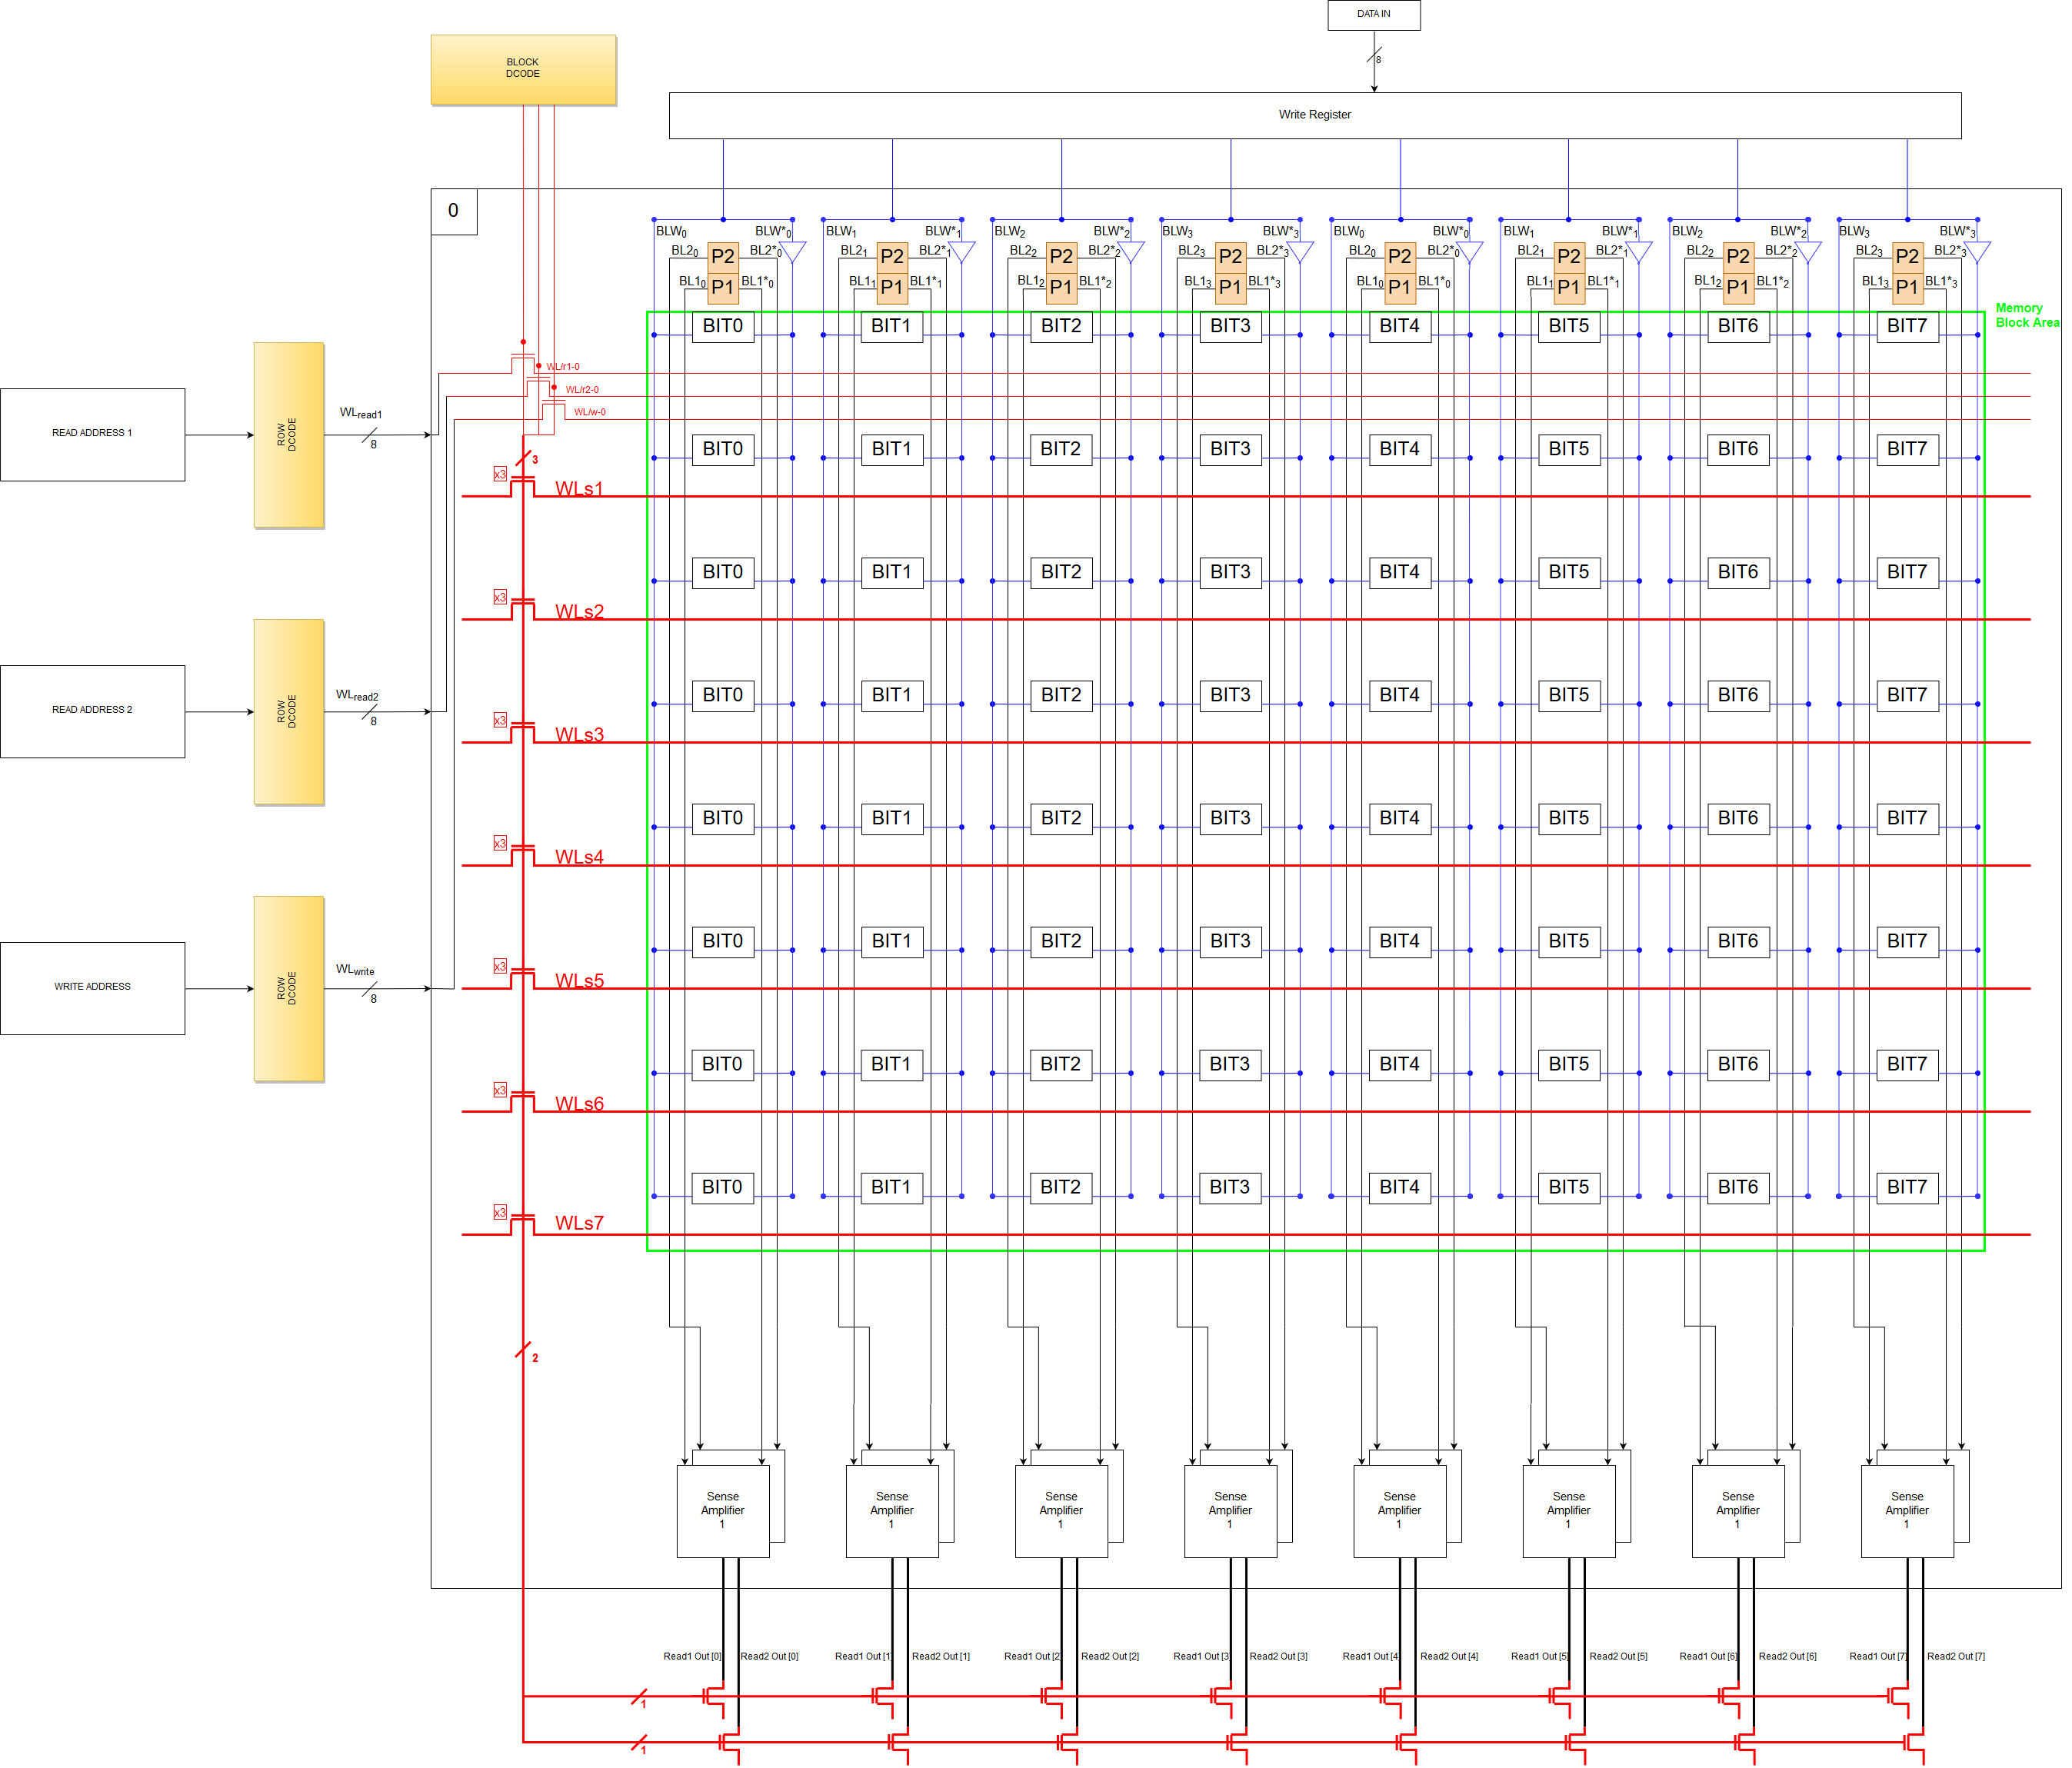
\includegraphics[width=0.85\textwidth]{REG_FILE-BLOCK_SCHEME.png}
	\end{center}
	\caption{Detailed structure of the register file} 
	\label{fig:REG_FILE-BLOCK_SCHEME}
\end{figure} 

\textbf{Write} operation. After having forced on all the bitlines in parallel the value to be written, the address of the word to be written is sent to the write block decoder and to the write row decoders (which, again, work together with the write block decoder); only the correct row decoder will activate the write wordline of the selected word, making all the memory cells connected to it store the value present on the bitlines. 

\section{Organization of the words}
As mentioned, each memory block has a width equal to the parallelism of a single word. In particular, since generally the producers of the memory chips try to make them as square as possible, for reasons of space availability on the boards, we decided to divide the $N_{word}$ words of parallelism $N_{bit}$ into exactly square blocks: for this reason the number of blocks inside the register file is computed like $$N_{block}=\left\lceil\frac{N_{word}}{N_{bit}}\right\rceil$$
where the number of rows in each block is equal to $$N_{wl}=min(N_{word},N_{bit})$$
Then of course the number of bits inside the block address and the row address can be computed like $$Block\ Address=\left\lceil log_2(N_{block})\right\rceil$$ $$Row\ Address=\left\lceil log_2(N_{wl})\right\rceil$$